\section{Analysis}

\subsection{Stakeholders}
    This project is designed with computer science education in mind. As such potential stake holders could include various educational institutions as well as individual teachers and tutors. For example, the project could be used in a sixth-form or university classroom to demonstrate the workings of the x86 architecture or the more general workings of a typical Von Neumann architecture CPU.

    In this particular instance, my stakeholder shall be my own A-Level computer science teacher, Mr. Sisley.

    \subsubsection{Interview} \label{sec:interview}
        My interview questions for Mr Sisley (stakeholder in education) are as follows:
        \begin{enumerate}
            \item Are you satisfied with the resources you currently have available for teaching about the low-level workings of computing systems?
            \item Have you considered implementing practical demonstrations into such lessons?
            \item If so, did you find that it enhanced the learning experience of your students?
            \item Have you before considered performing demonstrations using more simplistic, early computer systems (whether physical or emulated) to help illustrating your teaching points?
            \item What features would you look for in an emulator to make it most applicable for usage in a teaching environment?
            \item What would, in your opinion, be the ideal interface for such a piece of software?
        \end{enumerate}

        % TODO: Justify questions...

        My stakeholder expressed his current dissatisfaction with the teaching resources available for demonstrating the workings of low-level systems to students. He states that he is "only really aware of the little man computer simulation" which is "quite good for GCSE-level students". However, he does believe that is not really "suitable for A Level" and such feels there is a "gap in the market" for such a resource or piece of software. Indeed, this is something I hope to address with my project.

        Mr Sisley also stated that practical learning demonstrations are a "real benefit when trying to get an idea across to a class" due to low-level computing being a "very dry, abstract topic". Again he mentions the problems had with the little man computer simulation, stating that it "can be rather difficult for students to follow and understand". He later elaborates on ways in which my own solution can address these issues.

    \subsubsection{Stakeholder Requirements}
        Mr Sisley's requirements were assess by means of an interview (see section \ref{sec:interview} and appendix \ref{sec:full-interview}).

\subsection{Computational Methods}
    A computational solution is appropriate here for a number of reasons. One such reason is that one of the best ways for potential stake holders (i.e. teachers) to teach about the low-level workings of an x86 system is show some such system in action. While theoretically they could indeed source an old IBM PC or similar for this purpose, doing so nowadays is rather difficult and expensive due to the rarity of such old systems. Instead, a simpler alternative is to just run emulators of these old systems using their existing modern hardware. Another bonus of doing this as an alternative is that an emulator allows for far more precise information about and control of the running of the system. Indeed, this is a key aspect that I think will allow my project specifically to be useful in the domain of education as a key focus of its design is allowing for the exposure of the inner workings of the emulated system.

    \subsubsection{Abstraction}
        Abstraction is used in the project in the sense that not all of the many features of the Intel 8086 are actual implemented as they are superfluous for the purpose of this project. In particular, the entire concept of concept of the 8086 being a physical chip with specific pins is entirely disregarded as implementing such low-level emulation would be effectively pointless. The idea of transmitting data to memory via an address bus and a data bus is also abstracted away, with the emulator instead simply having a reference to an object representing main memory which is used for interaction with emulator memory. Hardware modes (\textit{min}, \textit{max} mode) are also unnecessary due to the aforementioned.

    \subsubsection{Decomposition}
        One conclusion I reached straight away was that the GUI and the emulator itself should be entirely decoupled and separated as much as possible. Decomposing the entire project into these two primary components was advantageous for a couple of reasons. Firstly, it allowed my to initially focus exclusively on the implementation of the emulator without getting bogged down with to implementing GUI simultaneously. In addition, it also allowed the emulator to run without a GUI at all which would be convenient for testing via automatic unit testing. From a future-proofing perspective, it could also allow for implementation of a CLI or additional GUIs using preferred GUI libraries for certain platforms.

        See figure \ref{fig:decomp} below for a detailed breakdown of the components this project is comprised of. This diagram was created using the divide \& conquer method of decomposition.

        \begin{figure}[h]
            \centering
            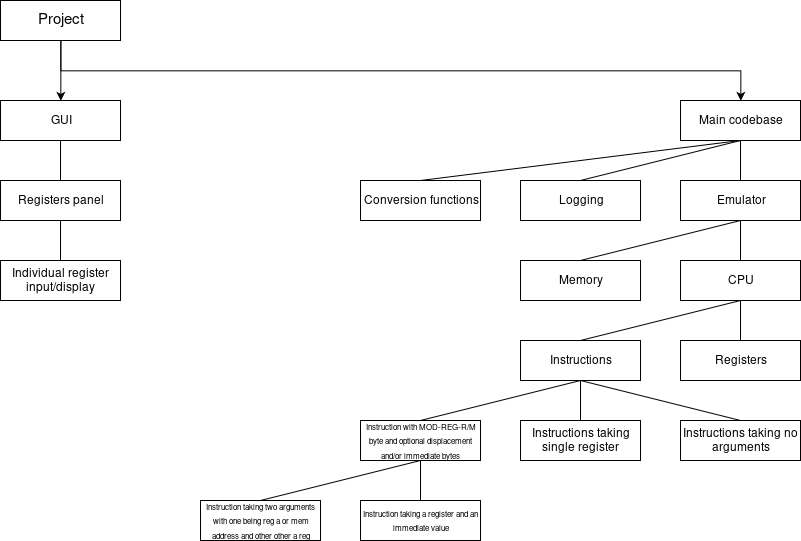
\includegraphics[width=0.8\textwidth]{decomposition}
            \caption{Decomposition of the project.}
            \label{fig:decomp}
        \end{figure}

    \subsubsection{Object-Orientation}
        I feel as though an emulator is particularly appropriate to an object-orientated design for a number of reasons. A computer system tends to have a set collection of components with each having a distinct function. The functioning of the system as a whole is then but a product of the interactions between these separate components. This lends itself well to an object-orientated design as each component of the emulated system (the CPU, memory, registers, etc.) can be implemented as a class with private internals and then a public interface to facilitate the interaction with other components.

        The ability to set private, protected and public properties of a class also encourages better design by limiting which pieces of code may modify certain variables or access certain methods. This is applicable to this particular project as being able to identify where program state is changed is integral to maintaining the stability of the program due to the fact that an emulator has many keepers of state that when modified dramatically influence its running (segment registers, CPU flags, among others).

        Object-orientated inheritance will also prove vital to allowing code reuse. In particular, classes to represent CPU instructions will benefit from inheritance especially due to the many subtypes of instruction having similarities to and sharing components of more general instruction types (see figures \ref{fig:hierarchy} and \ref{fig:decomp}).

        \begin{figure}[h]
            \centering
            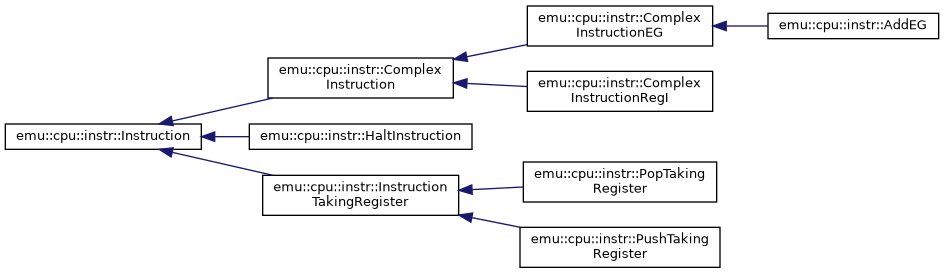
\includegraphics[width=0.8\textwidth]{hierarchy}
            \caption{Hierarchy of instruction classes.}
            \label{fig:hierarchy}
        \end{figure}

\subsection{Features \& Limitations}
    One feature that was required as part of the coursework specification was a Graphical User Interface (GUI). The choice of GUI library to use proved to be more challenging than anticipated - see section \ref{...} of the Design portion of this document for more information.

    As stated above, one key feature of the emulator should be its applicability to a teaching environment. As such, detailed information regarding the running of the emulator (state of registers, assembly expression of the current instruction, state of main memory, etc.) should be readily available. In addition, ability to modify the state of emulator should be possible to allow students to learn through the observing the consequences of any modifications they make. On the topic of modification, the source code of the project must be well organised, cleanly written, and fully documented so that students may learn through reading its implementation and by potentially making modifications to the software itself.

    Speed of execution is most certainly not to be prioritised during development meaning any optimisations that could be made to the code at the expense of readability or stability are not to be made. This lack of optimisation could potentially be presented as a limitation of the software in certain situations. However, due to emulation of such old hardware not being particularly resource-intensive as well as the project being implemented in the fast, compiled C++ language, this should not present any significant issues.

    Another limitation of the solution is that fact that not all of the instructions of the Intel 8086 can be run on it (see appendix section \ref{sec:instructset}). This means that complex programs that utilise more obscure instructions will be not be able to run on the emulator system. Fortunately, this should not cause significant issues due to the fact that software aimed primarily at teaching does not require advanced/obscure features.

\subsection{Software \& Hardware Requirements}
    \subsubsection{Hardware}
        The software will have only one real hardware requirement: a computer. This computer should have a architecture which can be targeted by the chosen compiler (see section \ref{sec:software-require}). At least 2 GB of DDR3 RAM is recommended (depending on the OS used).

    \subsubsection{Software} \label{sec:software-require}
        In terms of running the software, the only requirement is an operating system with a graphical desktop environment/window manager that supports the creation of and interaction with an SFML window.

        As for compilation, there are several software requirements. The first of such requirements being CMake version 3.12 or higher. The purpose of this software is to generate an appropriate build system using whatever is available on the system. As such, appropriate software that CMake can use to handle the actual compilation process is also required. On my Linux system, CMake uses the GCC, GNU Linker, and Make programs which I also have installed. On Windows, it uses Microsoft Visual C++ for compilation. CMake will produce an error message if no appropriate compiler/build system is installed. The project's \texttt{CMakeLists.txt} file specifies that C++ Standard 17 is required and so will also produce an error message should the available compiler not support that version of C++ (for example, all features of C++ 17 are implemented in GCC version 8 and above).

        Compiling the software also requires that a few libraries are installed for the purpose of creating a GUI. These include: SFML, ImGUI, and the SFML binding for ImGUI. The project also uses the Catch2 library for unit testing, however this only requires a single header file which is to be distributed with the project's source code and as such requires no additional installation steps.

\subsection{Existing Projects}
    \subsubsection{i8086emu}
        \begin{figure}[h]
            \centering
            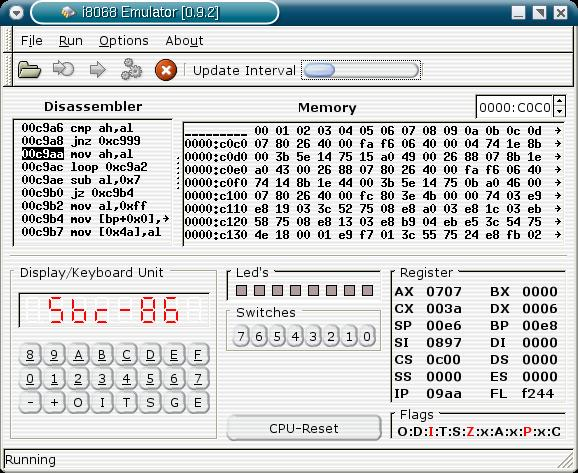
\includegraphics[width=0.8\textwidth]{i8086emu}
            \caption{Screenshot of the i8086emu emulator's GUI.}
            \label{fig:i8086emu}
        \end{figure}

        There are a few different existing emulators of the Intel 8086 microprocessor and associated hardware. One such existing project goes by the name of \textit{i8086emu}. As seen in figure \ref{fig:i8086emu}, this emulator has some some interesting features that I ultimately decided to implement into my own emulator. For example, one feature of i8086emu is its disassembler. This displays the instructions that the CPU has and will execute in a human-readable assembly format. I felt such a feature would be important to add to my own emulator as it gives the user convenient insight into what each instruction in memory will do without having to manually perform opcode and MOD-REG-R/M lookups. This makes the software especially applicable to a teaching environment as it provides a basic demonstration of CPU instruction decoding.

        The i8086emu emulator also shows the value of CPU registers and flags as part of its user interface. Again, such a feature would be vital to include in my emulator as it provides vital insight into the running of the emulation. However, I also decided to go a step further and allow the user to modify the values of registers via the interface during execution. This facilitates students using the emulator to experiment with and hopefully learn through observing results after changes are made to register values.

        While the code of the i8086emu is fairly readable and commented consistently, all of those comments are written in German. As such, learning through the reading and modification of the source code may prove challenging for students unable to read German. Naturally, I hope to improve on this by providing clear comments in English in my own emulator.

        The i8086emu project source code is listed under the GNU General Public License (GPL) which means that its code is free to be modified and redistributed while requiring any modifications are also licensed under the GPL. As someone who appreciates open-source software and have found it invaluable over the years, I feel a desire to also use a similar such license for my own project.

\subsection{Success Criteria}
    The original success criteria of this project was far too ambitious given the limited time available to be dedicated to this project. Originally, it was planned that the emulator would be considered complete only once it was capable of running a Basic Input Output System (BIOS) and then successfully booting an early version of Microsoft Disk Operating System (MS-DOS). While this of course would have been rather impressive, it would have required an entirely bug-free implementation of the entirety of the Intel 8086, Intel 8259 Programmable Interrupt Controller, Intel 8253 Programmable Interval Timer, etc.

    As for more realistic, concrete success criteria, a few points have since been decided upon. These are outlined in the subsections below.

    \subsubsection{GUI}
        The GUI must fulfil the following criteria:
        \begin{itemize}
            \item Must display values of CPU registers as well as allow for the altering of said values during execution by the user.
            \item Must display the assembly representation of the instruction currently being executed.
            \item Allow for the loading of raw data files in emulator memory via a menu option.
        \end{itemize}

    \subsubsection{Emulator}
        The emulator must fulfil the following criteria:
        \begin{itemize}
            \item Capable of executing all instructions listed in appendix section \ref{sec:instructset} successfully including cases where those instructions may include MOD-REG-R/M, immediate and/or displacement bytes.
            \item Capable of producing correct assembly representations of all instructions listed in appendix section \ref{sec:instructset}.
            \item Does not crash when provided with an unknown/unimplemented opcode or instruction with invalid encoding.
        \end{itemize}
